\documentclass[slidetop,11pt]{beamer}

% Ces deux lignes � d�commenter pour sortir
% le texte en classe article
% \documentclass[class=article,11pt,a4paper]{beamer}
% \usepackage{beamerbasearticle}

% Packages pour les fran�ais
%
\usepackage[T1]{fontenc}
\usepackage[latin1]{inputenc}
\usepackage[frenchb]{babel}
% pour un pdf lisible � l'�cran si on ne dispose pas
% des fontes cmsuper ou lmodern
%\usepackage{lmodern}
\usepackage{aeguill}

% Pour afficher le pdf en plein ecran
% (comment� pour imprimer les transparents et pour les tests)
%\hypersetup{pdfpagemode=FullScreen}

% ------------------------------------------------
%-----------   styles pour beamer   --------------

% Supprimer les icones de navigation (pour les transparents)
\setbeamertemplate{navigation symbols}{}

\setbeamertemplate{footline}
{
\hfill\insertframenumber/\inserttotalframenumber~~~
}

% Mettre les icones de navigation en mode vertical (pour projection)
%\setbeamertemplate{navigation symbols}[vertical]

% ------------ Choix des th�mes ------------------

%\usetheme{Boadilla}
%\usetheme{Goettingen}
%\usetheme{Hannover}
%\usetheme{Marburg}
%\usetheme{Warsaw}
\usetheme{Frankfurt}

%------------ fin style beamer -------------------

\title{Ecosystem Dynamics for Creative Image Generation}
%\subtitle{}
\author{Andr�a Machizaud, Stefan Bornhofen and Vincent Gardeux}
\institute{L@ris, EISTI}
\date{ICSI'11 - June 14,15, 2011}

% ------------------------------------------------
% -------------   D�but document   ---------------
% ------------------------------------------------
\begin{document}
%--------- �criture de la page de titre ----------
% avec la commande frame simplifi�e
\frame{\titlepage}
%
%------------------ Sommaire ---------------
\begin{frame}{Outline}
  \small \tableofcontents[hideallsubsections]
\end{frame}
%
%***************************************
%******     Les slides          *******
%***************************************

\section{Introduction}

%\subsection{Artificial Life}
%
%\begin{frame}
%\frametitle{Artificial Life}
%%Artificial Life is a field of study which goal is to study natural's phenomena in order to have a better understanding of complex interactions which rules such a system, and thus in the other hand make the most of those results to enhance actual concepts.\\
%%Experiments tend to focus on capturing most essentials concepts of a living system and implements them in an artificial environment to both observe expected concepts and inject some new rules.\\
%%Among class of experiments, agent based systems provide a solution based on observing emergent properties of societies of agents to understand the final result.
%
%\begin{itemize}
%    \item Understanding of natural system's complex interactions.
%    \item Enhance actual concepts inspired by natural's phenomena observation.
%    \item Capture fundamental concepts and inject new rules in an custom artificial environment.
%    \item Agent based systems observe emergent properties of a society of agents.
%\end{itemize}
%
%\end{frame}

\subsection{Ecosystem Art}

\begin{frame}
    \frametitle{Ecosystem Art}
\begin{block}{\textbf{Context}}
    \begin{itemize}
        \item Blend between art and science
        \item Agent based system
        \item Emergent pattern resulting in an artistic result
        \item Constant innovation, investigate further ideas
    \end{itemize}
\end{block}
\end{frame}

\begin{frame}
    \frametitle{Ecosystem Art}
%\begin{block}{\textbf{Previous studies}}
    \begin{table}{c}
  % Requires \usepackage{graphicx}
  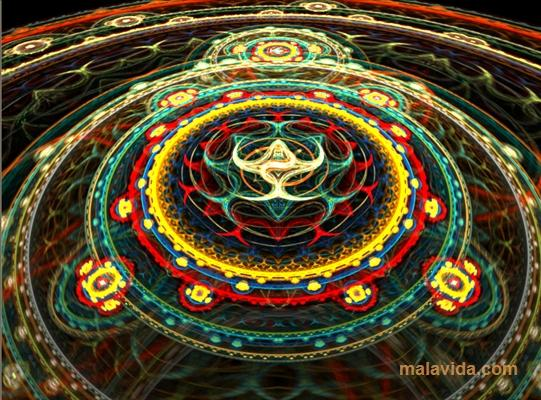
\includegraphics[width=30px]{electric-sheep.jpg}\\
    \end{table}
%\end{block}
\end{frame}

\begin{frame}
    \frametitle{Ecosystem Art}
\begin{figure}
    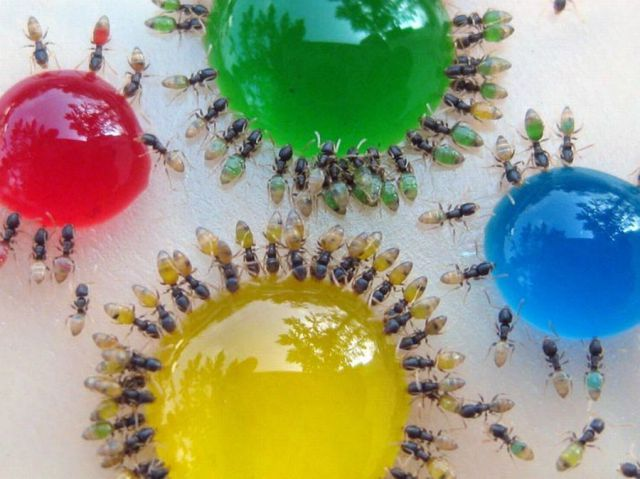
\includegraphics[height=150px]{creative-ecosystem}
\end{figure}
\end{frame}

\section{Model}

\subsection{General Principle}

\begin{frame}
    \frametitle{General Principle}
\begin{itemize}
\item toto
\item titi
\end{itemize}
\end{frame}


\subsection{Phenotype}

\begin{frame}
    \frametitle{Phenotype}
\begin{itemize}
\item bla
\item bla
\item bla
\end{itemize}
\end{frame}

\subsection{Genotype}

\begin{frame}
    \frametitle{Genotype}
\begin{block}{\textbf{Parameters}}
    \begin{itemize}
        \item curvature : ...
        \item irrationality : ...
    \end{itemize}
\end{block}

\end{frame}

\subsection{Behavior}

\begin{frame}
    \frametitle{Behavior}
\begin{block}{\textbf{Hunting}}
    \begin{itemize}
        \item bla
        \item bla
    \end{itemize}
\end{block}

\begin{block}{\textbf{Feeding}}
    \begin{itemize}
        \item bla
        \item bla
    \end{itemize}
\end{block}

\end{frame}

\subsection{Coloration}

\begin{frame}
    \frametitle{Coloration}
\begin{itemize}
\item color
\end{itemize}
\end{frame}

\section{Experiments}

\subsection{Basic Experiment}

\begin{frame}
    \frametitle{Basic Experiment}
\begin{itemize}
\item t
\item t
\end{itemize}
\end{frame}


\section{Discussion}

\subsection{Coloration}

\begin{frame}
    \frametitle{Coloration}

\begin{itemize}
\item eee
\item eee
\item eee
\end{itemize}

\end{frame}

\section{Conclusion}

\subsection{Conclusion}

\begin{frame}
    \frametitle{Conclusion}
    \begin{itemize}
    \item Nos r�sultats surpassent les autres
    \item R
    \item C'est beau!
    \end{itemize}
\end{frame}

\subsection{Extending Works}

\begin{frame}
    \frametitle{Extending Works}
    \begin{itemize}
	\item L
	\item Fon
	\item Fon
    \item A
    \end{itemize}
\end{frame}

\begin{frame}
 	\begin{block}{ }
		\center Thank you for your attention.\\
		\center Any questions ?
	\end{block}
	\begin{center}
		Vincent Gardeux\\
		Enseignant-chercheur EISTI\\
		Doctorant de l'Universit� Paris-Est Cr�teil
	\end{center}

	\begin{center}
		Davantage d'informations � propos des recherches en cours :\\
		\underline{http://gardeux-vincent.eu}
	\end{center}
\end{frame}

\end{document}
